\documentclass{amsart}
\usepackage{xcolor,tikz}
\usetikzlibrary[positioning]

\begin{document}

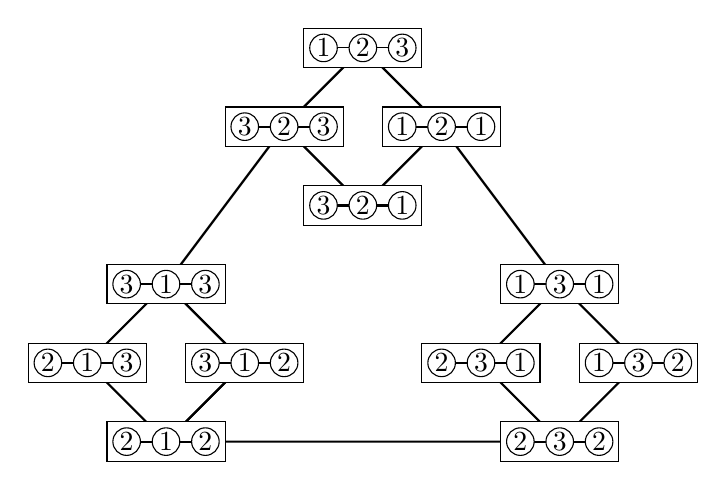
\begin{tikzpicture}[baseline=0cm, scale=0.5]

% top square 
\node (a) at (0,0) {};
\node (b) at (-2,-2) {};
\node (c) at (0,-4) {};
\node (d) at (2,-2) {};
\node (e) at (-5,-6) {};
\node (f) at (5,-6) {};
\draw[style=thick] (b)--(e)--(-3,-8)--(-5,-10)--(5,-10)--(7,-8)--(5,-6)--(d);
\draw[style=thick] (e)--(-7,-8)--(-5,-10);
\draw[style=thick] (5,-6)--(3,-8)--(5,-10);
\draw[style=thick] (-5,-6)--(-3,-8)--(-5,-10);
\draw[style=thick] (a)--(b)--(c)--(d)--(a);
\draw[fill=white] (-1.5,-.5) rectangle (1.5,.5);
\draw[fill=white](-1,0)--(1,0);
\draw[radius=.35,fill=white](-1,0)circle node {1};
\draw[radius=.35,fill=white](0,0)circle node{2};
\draw[radius=.35,fill=white](1,0)circle node{3};

\draw[fill=white] (-3.5,-2.5) rectangle (-.5,-1.5);
\draw[style=thick](-3, -2)--(-1,-2);
\draw[radius=.35,fill=white](-3,-2)circle node{3};
\draw[radius=.35,fill=white](-2,-2)circle node{2};
\draw[radius=.35,fill=white](-1,-2)circle node{3};

\draw[fill=white] (3.5,-2.5) rectangle (.5,-1.5);
\draw[style=thick](3, -2)--(1,-2);
\draw[radius=.35,fill=white](3,-2)circle node{1};
\draw[radius=.35,fill=white](2,-2)circle node{2};
\draw[radius=.35,fill=white](1,-2)circle node{1};

\draw[fill=white] (-1.5,-4.5) rectangle (1.5,-3.5);
\draw[style=thick](-1,-4)--(1,-4);
\draw[radius=.35,fill=white](-1,-4)circle node{3};
\draw[radius=.35,fill=white](0,-4)circle node{2};
\draw[radius=.35,fill=white](1,-4)circle node{1}; 

% left square

\draw[fill=white] (-6.5,-6.5) rectangle (-3.5,-5.5);
\draw[style=thick](-6,-6)--(-4,-6);
\draw[radius=.35,fill=white](-6,-6)circle node{3};
\draw[radius=.35,fill=white](-5,-6)circle node{1};
\draw[radius=.35,fill=white](-4,-6)circle node{3};

\draw[fill=white] (-8.5,-8.5) rectangle (-5.5,-7.5);
\draw[style=thick](-8, -8)--(-6,-8);
\draw[radius=.35,fill=white](-8,-8)circle node{2};
\draw[radius=.35,fill=white](-7,-8)circle node{1};
\draw[radius=.35,fill=white](-6,-8)circle node{3};

\draw[fill=white] (-4.5,-8.5) rectangle (-1.5,-7.5);
\draw[style=thick](-2, -8)--(-4,-8);
\draw[radius=.35,fill=white](-2,-8)circle node{2};
\draw[radius=.35,fill=white](-3,-8)circle node{1};
\draw[radius=.35,fill=white](-4,-8)circle node{3};

\draw[fill=white] (-6.5,-10.5) rectangle (-3.5,-9.5);
\draw[style=thick](-6,-10)--(-4,-10);
\draw[radius=.35,fill=white](-6,-10)circle node{2};
\draw[radius=.35,fill=white](-5,-10)circle node{1};
\draw[radius=.35,fill=white](-4,-10)circle node{2}; 

% right square

\draw[fill=white] (3.5,-6.5) rectangle (6.5,-5.5);
\draw[style=thick](4,-6)--(6,-6);
\draw[radius=.35,fill=white](4,-6)circle node{1};
\draw[radius=.35,fill=white](5,-6)circle node{3};
\draw[radius=.35,fill=white](6,-6)circle node{1};

\draw[fill=white] (1.5,-8.5) rectangle (4.5,-7.5);
\draw[style=thick](2, -8)--(4,-8);
\draw[radius=.35,fill=white](2,-8)circle node{2};
\draw[radius=.35,fill=white](3,-8)circle node{3};
\draw[radius=.35,fill=white](4,-8)circle node{1};

\draw[fill=white] (5.5,-8.5) rectangle (8.5,-7.5);
\draw[style=thick](8, -8)--(6,-8);
\draw[radius=.35,fill=white](6,-8)circle node{1};
\draw[radius=.35,fill=white](7,-8)circle node{3};
\draw[radius=.35,fill=white](8,-8)circle node{2}; 

\draw[fill=white] (3.5,-10.5) rectangle (6.5,-9.5);
\draw[style=thick](4,-10)--(6,-10);
\draw[radius=.35,fill=white](4,-10)circle node{2};
\draw[radius=.35,fill=white](5,-10)circle node{3};
\draw[radius=.35,fill=white](6,-10)circle node{2}; 
\end{tikzpicture}

\end{document}